\documentclass{article}
\usepackage{graphicx}
\usepackage[margin=1.5cm]{geometry}
\usepackage{amsmath}

\begin{document}

\title{Tuesday Reading Assessment: Chapter 3-1 through 3-3}
\author{Prof. Jordan C. Hanson}

\maketitle


\section{Basic Logic Gates}

\begin{enumerate}
\item
\begin{figure}[ht]
\centering
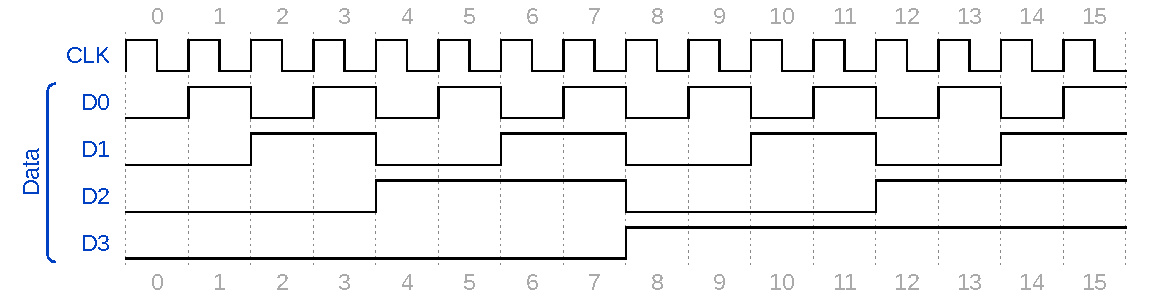
\includegraphics[width=0.6\textwidth]{figures/timingExample14.pdf}
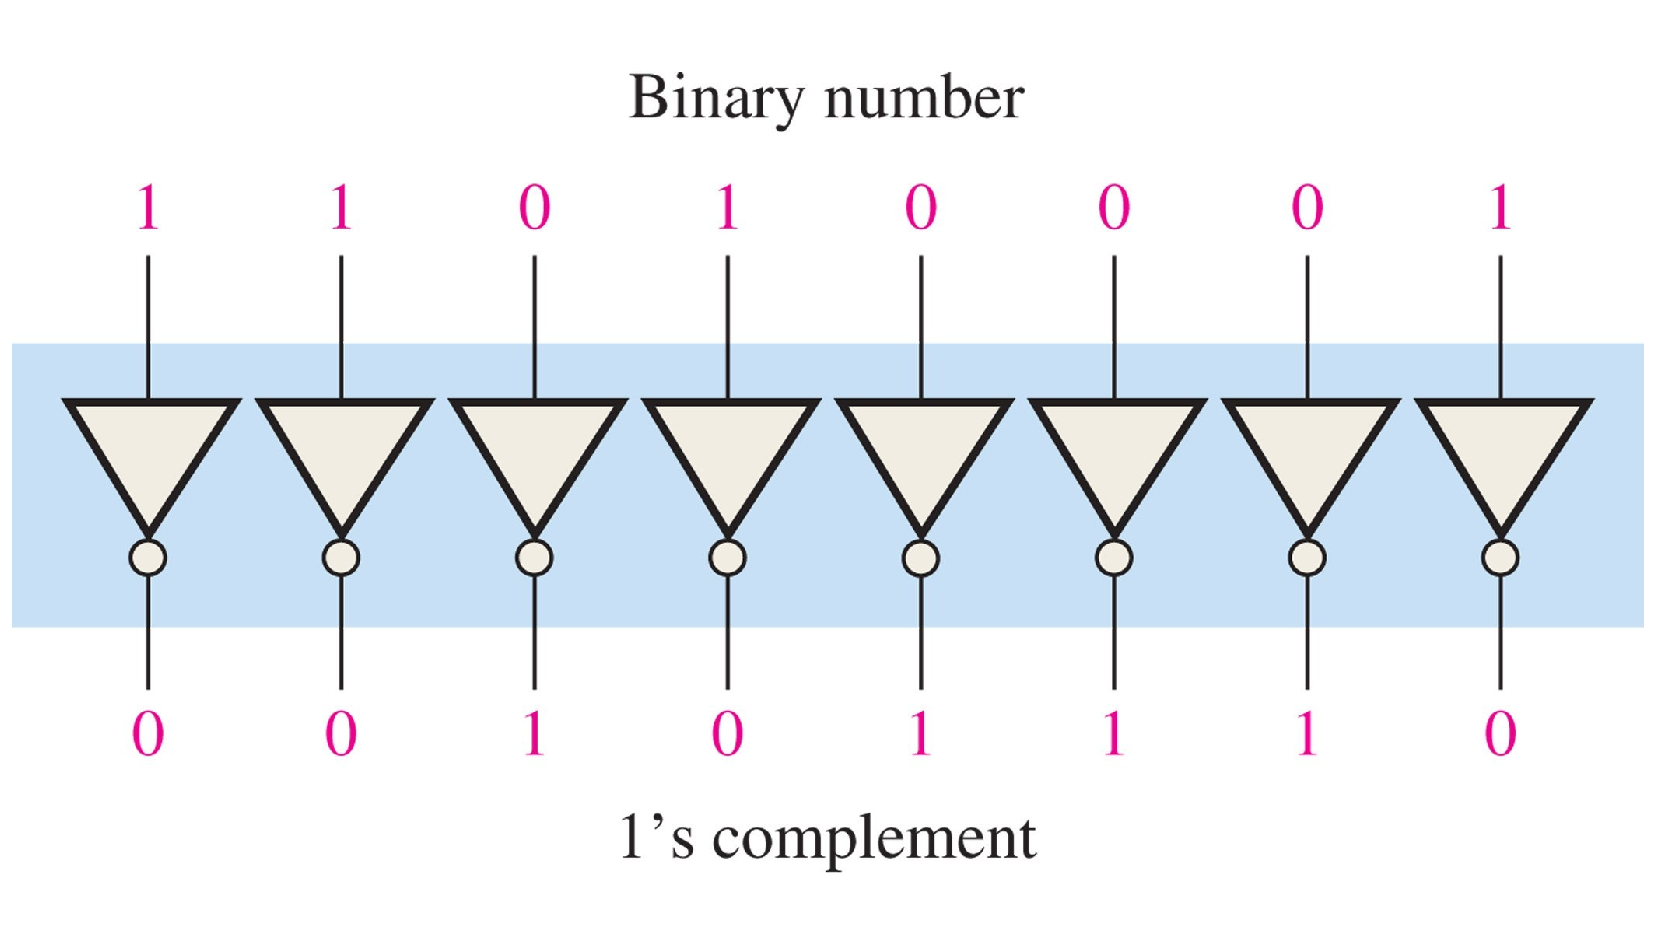
\includegraphics[width=0.35\textwidth]{figures/ones_c.pdf}
\caption{\label{fig:ones} (Left) A timing diagram for a 4-bit parallel binary number.  (Right) A simple logic circuit that computes the ones complement of a byte in parallel.}
\end{figure}
Consider Fig. \ref{fig:ones}, in which a 4-bit parallel data stream is shown (right), and a basic logic circuit is shown (left).
\begin{itemize}
\item Describe in words what function or process is happening with the data bits D0-D3 in Fig. \ref{fig:ones} (left). \\ \vspace{0.5cm}
\item Suppose D0-D4 were fed into the left-most gates in Fig. \ref{fig:ones}.  Draw the timing diagram below. \\ \vspace{2cm}
\end{itemize}
\item 
\begin{figure}
\centering
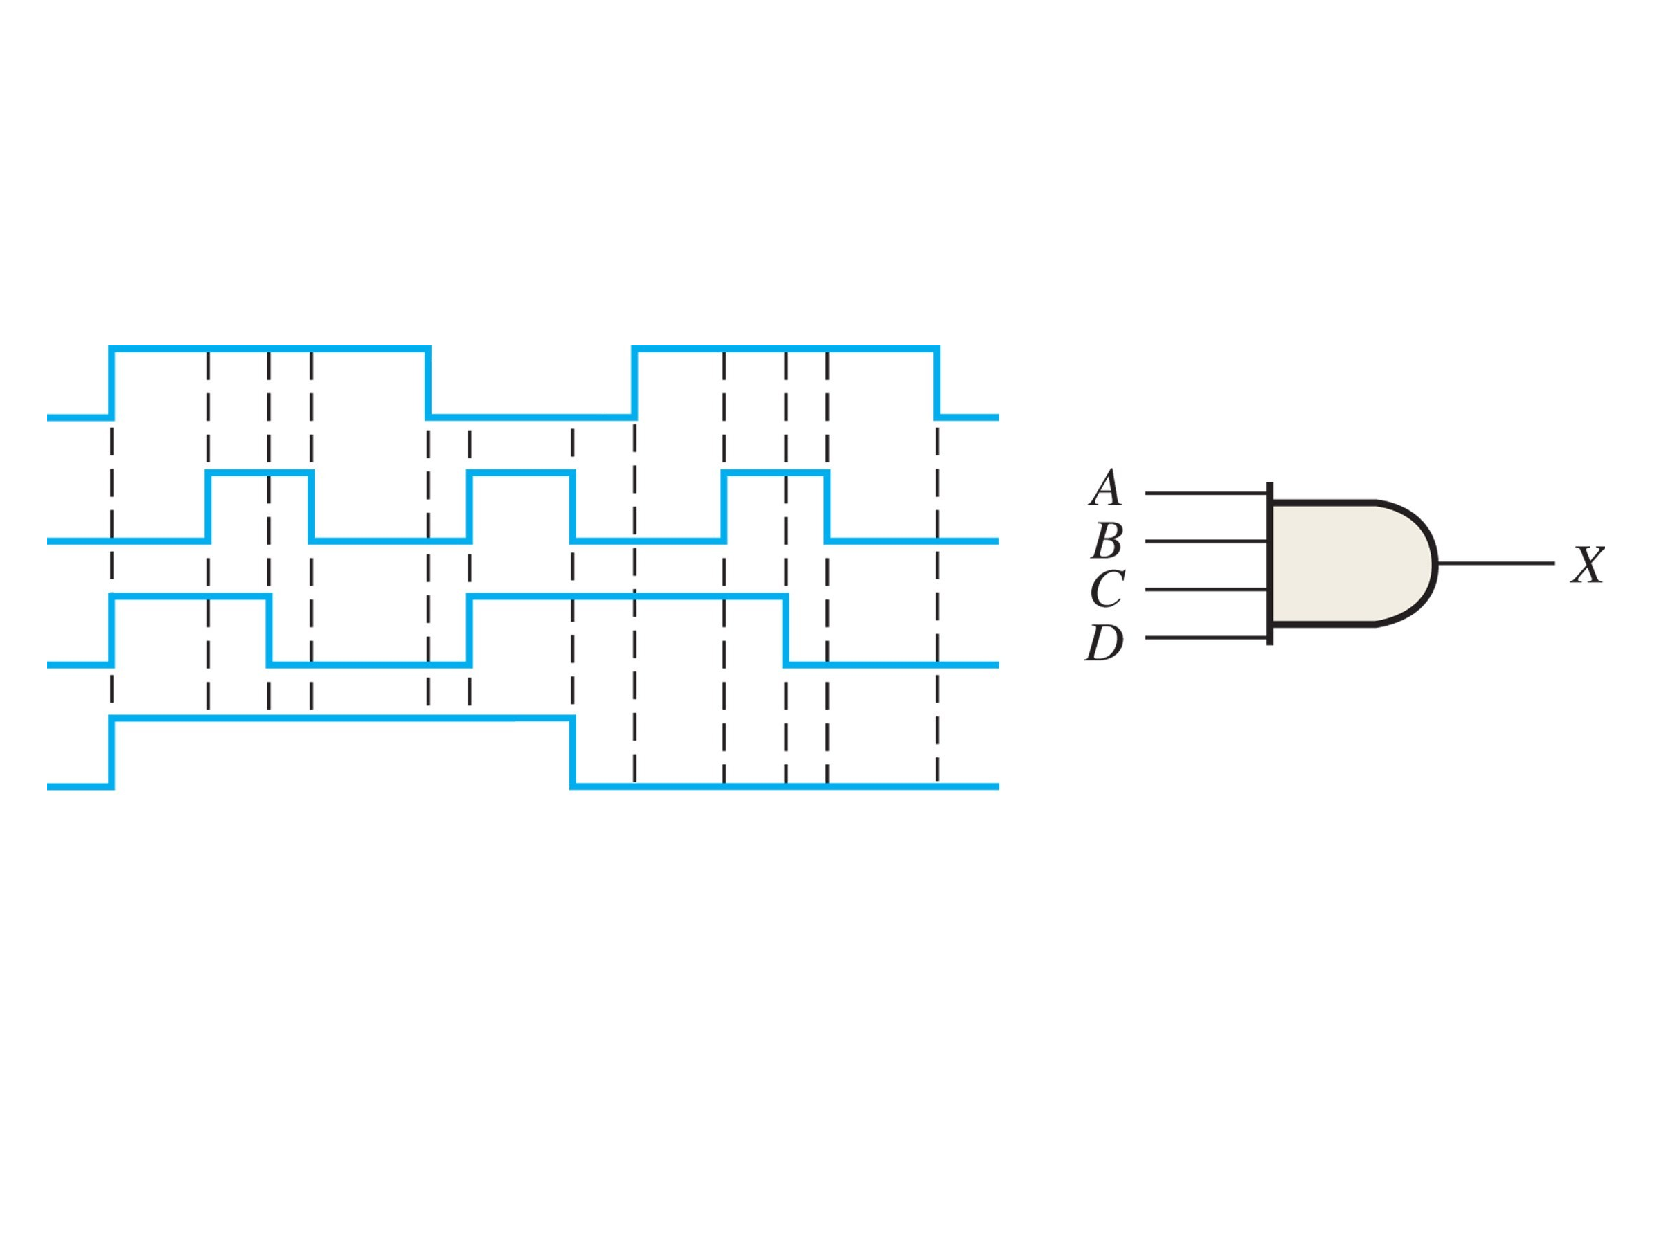
\includegraphics[width=0.5\textwidth,trim=0cm 4cm 0cm 4cm,clip=true]{4and.pdf}
\caption{\label{fig:4and} A timing diagram as input to a 4-input AND gate.}
\end{figure}
Draw the output timing diagram for the 4-input AND gate below.  \textit{Hint: what should the truth table be for the 4-input AND?}
\end{enumerate}

\end{document}
